%
% CHAPTER: Entities, Represenations and Descriptions
%

\chapterimage{owl.pdf} % Chapter heading image

\chapter{Entities, Representations and Descriptions}
\label{cha:Topics-and-Descriptions}

\begin{quote}
\begin{flushright}
\emph{We are all agreed that your theory is crazy. \\
The question which divides us is whether it is crazy enough.} \\
Niels Bohr
\end{flushright}
\end{quote}
\bigskip

The first step to quantitatively measure how much we do not know is to identify clearly the collection of research entities under study. The exact elements of this collection is something that depends on the particular application in which the theory of nescience is being used. Different applications require different collections of entities (mathematical objects, living things, human needs, etc.). Fortunately, the procedure to compute how much we do not know is the same in all cases.

The second step is to provide a method to encode the set of identified entities as strings of symbols, what we call representations. How to properly encode a research entity with symbols is a difficult, still unsolved, epistemological problem. The solution we propose in the theory of nescience is based in the concept of oracle Turing machine. How easy is to implement this solution in practice is something that depends on how abstract are the entities under study. For example, the collection of all abstract mathematical objects is a very difficult set to encode, and so, an approximation has to be found; the collection of all possible computer programs (given that our area of interest is software quality, see Chapter \ref{chap:Software-Engineering}) is far easier to encode, since computer programs are strings themselves.

The final step, once we have found a way to properly encode the original set of entities as string-based representations, is to provide a description, as accurate and succinct as possible, of what we already know about those representations. In the theory of nescience we require that descriptions must be computable, that is, given a description, a computer should be able to fully reconstruct the original representation. A difficult problem that arise with descriptions is that they characterize representations, that is, the encoding of entities, not the entities themselves, and so, the quality of a description for an entity is conditional to the quality of the representation used.

In this chapter we will formalize all these concepts: entities, representations, descriptions, and many others. We will also see what we mean by a perfect description, how to compute the combined representation of multiple entities, and the description of a representation assuming a perfect description of another one. The concept of research area, and its properties, will be also investigated.

%
% Section: Entities
%

\section{Entities}
\label{sec:descriptions_entities}

What exactly is a research entity is a difficult, still unsolved, philosophical problem. Our approach to address this complex issue is eminently practical. Our theory starts by assuming there exists a non-empty collection of \emph{entities}\index{Entities} we would like to understand.

\begin{notation}
We denote by $\mathcal{E}$ the set of research entities in which we are interested.
\end{notation}

The exact elements that compose $\mathcal{E}$ is something that depends on the particular domain in which the theory of nescience is being applied, but they usually corresponds to an area of knowledge. Examples of sets of entities could be: research elements in mathematics (abstract); the kingdom of animalia (living things); known and unknown human needs (abstract); all possible computer programs (strings), etc. Technically speaking $\mathcal{E}$ is not a well defined set, since in general we cannot tell what is and what is not a member of this set.

The abstract nature of $\mathcal{E}$ has some advantages, but also introduces important limitations. The main limitation is that our definition of nescience is, in general, a non-computable quantity, and so, it must be approximated in practice. The main advantage is that we can apply the new concepts and methods introduced in this book to other problems, not only to the discovery of new scientific knowledge.

In the theory of nescience we do not allow universal sets, that is, we cannot assume the existence of a set $\xi$ that contains everything. The problem with universal sets is that they violate Cantor's theorem (see Example \ref{cantor_theorem}). Cantor's theorem states that the power set $\mathcal{P}(\xi)$ composed by all the possible subsets of $\xi$ has more elements than the original set $\xi$, and this is a contradiction with the fact that $\xi$ contains everything. In the theory of nescience the set $\mathcal{E}$ must be the set of something.

\begin{example}[Cantor's theorem]
\label{cantor_theorem}
The Cantor's theorem states that for every set $A$ we have that $d(A) < d\left(\mathcal{P}(A)\right)$. Let $f: A \rightarrow \mathcal{P}(A)$ a function that maps every element of $x \in A$ to the set $\{x\} \in \mathcal{P}(A)$; clearly $f$ is injective, and so, $d(A) \leq d\left(\mathcal{P}(A)\right)$. In order to prove that the inequality is strict assume there exist a surjective function $g: A \rightarrow \mathcal{P}(A)$, and consider the set $B = \{ x \in A : x \notin g(x) \}$. Since $g$ is surjective there must exists an $y \in A$ such that $g(y) = B$. However this rises the contraction $y \in B \Leftrightarrow y \notin g(y) = B$. Consequently, the function $g$ does not exists, and so $d(A) < d\left(\mathcal{P}(A)\right)$.
\end{example}

Not all possible sets are valid sets in the theory of nescience, because some sets lead to paradoxes. For example, the Russel paradox propose to consider the set $R$ composed by all those sets that are not members of themselves; the paradox arises when we try to answer the question of whether $R$ is a member of itself (see Example \ref{ex:russell_paradox}). In order to avoid these kind of problems, the theory of nescience is based on the Zermelo-Fraenkel set of axioms together with the axiom of choice (see Appendix \ref{apx:math}). Russell's paradox is due to an abuse of the set builder notation $\{ : \}$. The \emph{axiom of separation} (if $P$ is a property with parameter $p$, then for any set $x$ and parameter $p$ there exists a set $y=\{u \in x : P(u) \}$ that contains all those sets $u \in x$ that have property $P$) only allows the use of this notation to construct sets that are subsets of already existing sets. A more general \emph{axiom of comprehension} (if $P$ is a property, the there exist a set $y=\{u : P(u) \}$) would be required to allow sets like the one proposed by Russell's paradox. In the ZFC axioms, and in the theory of nescience, the axiom of comprehension is considered to be false.

\begin{example}[Russell's Paradox]
\label{ex:russell_paradox}
Let $R$ be the set composed by all sets that are not members of themselves, that is, $R = \{ x : x \notin x \}$. The contradiction arises when we ask if $R$ is member of itself. If $R$ is not a member of itself, according to its own definition it should be; however if we say that $R$ is a member of itself, the definition tell us that it should not be. Symbolically $R \in R \Leftrightarrow R \notin R$.
\end{example}

In the theory of nescience we do not deal with classical ontological questions, that is, about the classes of things that there exists in the world and that can be known. Also, we do not try to answer any kind of epistemological issues, like for example, how scientific knowledge is validated by appeal to evidence, or what it is the nature of that evidence.

Once we have selected a set $\mathcal{E}$ of entities, the next step is to uniquely encode their elements as strings of symbols, otherwise it would not be possible to describe them (unless entities are strings of symbols themselves). How to properly perform this encoding is described in the next section.

%
% Section: Representations
%

\section{Representations}
\label{sec:representations}

How to represent the, possibly abstract, entities of a set $\mathcal{E}$ is a difficult epistemological problem that has been the subject of research for more than two thousand years (see Section \ref{sec:scientific_representation} for a short review of difficulties and open questions). In this book we describe a possible solution to this problem, and we will study its advantages and drawbacks. We propose to split the scientific representation problem it two complementary subproblems: how descriptions model representations, and how representations encode entities. In this sense, scientific descriptions are characterizations of entities by virtue of an indirect relation through representations (recall Figure \ref{fig:representationProblem} in the introduction of this book, reproduced again below for an easier reference). In this section we will focus on the encoding part, and Section \ref{sec:descriptions_models} will be about descriptions.

\begin{figure}[h]
\centering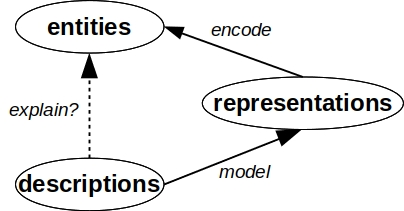
\includegraphics[scale=0.5]{representationProblem}
\caption{The Problem of Understanding.}
\end{figure}

In the discipline of Kolmogorov complexity, researchers solve the problem of representation by assuming that the set $\mathcal{E}$ is well defined, countable, and that there exists a total encoding function $f:\mathcal{E} \rightarrow \mathbb{N}$ from the set of entities to the set of natural numbers (a kind of Gödel numbering). In the theory of nescience we borrow this idea of encoding entities with numbers, or equivalently, strings of symbols. The main difference is that we address the problem of encoding an arbitrary set $\mathcal{E}$ by turning it around, that is, by defining a total function $\mathcal{O}_\mathcal{E}:\mathcal{S}^\ast \rightarrow \mathcal{E}$ from the well defined set $\mathcal{S}^\ast$ of all possible finite strings from an alphabet $\mathcal{S}$ to the, perhaps not countable and even not well defined, set $\mathcal{E}$ of entities under study.

Our function $\mathcal{O}_\mathcal{E}$, that depends on the set $\mathcal{E}$, is a kind of oracle (inspired by the concept of oracle Turing machine from Definition \ref{def:Oracle-Turing-Machine}) that is able to fully reconstruct an entity $\mathcal{O}_\mathcal{E} (x) \in \mathcal{E}$ given its encoding string $x \in \mathcal{S}^\ast$, without requiring additional information. Of course, this oracle is a conceptual idea that cannot be built in the real world for the majority of the sets $\mathcal{E}$, but assuming its existence will allow us to explain and prove important properties of how the process of scientific discovery works. $\mathcal{O}_\mathcal{E}$, being an oracle and not a regular function, is limited in terms of the mathematical operations in which it can used, as we will see below.

We assume that there exists a single, unique, physical world, that is independent of observers. We also assume that for some collections of entities $\mathcal{E}$ it is free of logical contradiction to assume the existence of an oracle $\mathcal{O}_\mathcal{E}$ (see the scientific representation problem in Section \ref{sec:scientific_representation}). Without any loss of generality, for the rest of this book we will only consider binary strings as encoding of entities.

\begin{definition}
\label{def:descriptions_topic}
Let $\mathcal{E}$ be a set of entities. A \emph{representation function} is an oracle $\mathcal{O}_\mathcal{E}:\mathcal{B}^\ast \rightarrow \mathcal{E}$ from the elements of the set $\mathcal{B}^\ast$ of all possible finite binary strings to the elements of the set $\mathcal{E}$ of entities under study.
\end{definition}

Only the elements of the set $\mathcal{B}^\ast$, that is, binary strings, can serve as representations of entities (problem of ontology). We do not allow drawings, or any other form of physical models, unless they are converted into binary strings. We do not make any distinction between a scientific representations and any other kind of representations (demarcation problem). It is up to the oracle to decide which entity is encoded by each representation. It is also important to note that the oracle $\mathcal{O}_\mathcal{E}$ is total, that is, all possible strings represent entities (no targetless models allowed).

\begin{example}
\label{ex:not_unique_oracle}
Given a set of entities $\mathcal{E}$, if a representation oracle $\mathcal{O}_\mathcal{E}$ exists, it is not unique. For example, a binary not oracle (transform the zeros of a binary string into ones and the ones into zeros) that assigns to each string $x \in \mathcal{B}^\ast$ the entity $\mathcal{O}_\mathcal{E} \left( \neg x \right)$ would be also a representation function.
\end{example}

We could have used an universal oracle machine instead of individual oracles. An universal oracle machine is a machine $\mathcal{U}_\mathcal{O}$ that given as input the encoding of an oracle $\mathcal{O}_\mathcal{E}$ and a string $s$, it computes $\mathcal{U}_\mathcal{O} \left( \langle \mathcal{O}_\mathcal{E}, s \rangle \right) = \mathcal{O}_\mathcal{E} \left( s \right)$. Universal machines make more sense when they are applied to the universal set $\xi$ that contains everything. However, that would make the the process of scientific discovery more difficult in practice. We prefer to work with a sets of entities $\mathcal{E}$ that correspond to particular areas of knowledge, and select one oracle $\mathcal{O}_\mathcal{E}$ for each set $\mathcal{E}$ (the best one according to our current knowledge).

\begin{example}
\label{ex:description_dna}
When the topics under study are animals we could start using as encodings a detailed description of the body of those animals. In this case, the oracle would be an hypothetical machine that given its description is able to reproduce the original animal. As we get a better understanding of the biology of life we can consider to use an alternative encoding based on the DNAs of the animals. Both encodings are valid representations of the entities.
\end{example}

We use an oracle function instead of an oracle relation $\mathcal{R}_\mathcal{O} \subset \mathcal{B}^\ast \times \mathcal{E}$, because our aim is not about matching strings with their correspoding entities, but building an entity given its representation. The capacity of the oracle of reconstruct the original entities is what justifies the fact that we can formulate hypotheses about entities given their representations (surrogative reasoning). According to the theory of nescience, scientific research would be not only about figuring out how to properly encode entities, but also about discovering the inner workings of the decoding oracles. 

The goal of encoding entities in the theory of nescience is different from that of Shannon's information theory, as Example \ref{ex:shannon_encoding} shows.

\begin{example}
\label{ex:shannon_encoding}
Consider a set $\mathcal{E}$ composed by two books, "The Ingenious Nobleman Sir Quixote of La Mancha" and "The Tragedy of Romeo and Juliet". We could encode the fist book with the string "0" and the second one with the string "1". Although those strings allow us to uniquely identify each book in the set, they are not proper encodings in the sense of the theory of nescience. Information theory is about how to uniquely identify an object given a reference and it requires that both, sender and received agree about a mapping between references and objects. Meanwhile, in the theory of nescience we are interested in how to provide a representation that captures all the details and nuances of the original objects. For example, given the strings "0" and "1" it is not possible to make any hypothesis about the influence of Cervantes in the work of Shakespeare.
\end{example}

An alternative way to deal with the problem described in Example \ref{ex:shannon_encoding}, where we used artificially short descriptions, would be to require the set $\mathcal{E}$ to be infinite, as Kolmogorov complexity does (we can not cheat an infinite number of times). However, even requiring the set of entities to be infinite, not every possible encoding schema can guarantee that the highly desirable property of surrogative reasoning is satisfied.

As it was shown in Example \ref{ex:not_unique_oracle} and Example \ref{ex:description_dna}, the entities of $\mathcal{E}$ might be encoded in multiple ways (problem of style). Different oracles will admit different encoding schemas. Some of those strings are better representations of an entity than others (standard of accuracy). Which representation is the best depends on the kind of questions we are interested to answer. In ant case, our aim should be to use those representations that make the size of the oracle (the amount of inner knowledge we assume the oracle contains) as small as possible.

Recall that the oracle is a total funcion, that is, all possible strings must represent an entity, including the incomplete ones. The more information is missing from a representation, the harder would be for us to understand how the oracle works. We must be careful with those representations that do not capture all the details about the original entities, since the results of our analyses could present some bias. In Chapter \ref{chap:Miscoding} we will study in detail the problem of errors due to the miscoding of abstract entities, and we will see that not only representations are about entities, but also we require that entities should be about representations (requirement of directionality).

\begin{example}
The data used in time of Ptolomeo about the position of celestial bodies along the year was a misencoding of the entity "position of celestial bodies". A better encoding was the data provided by Tycho Brahe. Today, we have even better encodings.
\end{example}

We distinguish between \emph{knowable} and \emph{unknowable} entities.

\begin{definition}
We say that an entity $e \in \mathcal{E}$ is \emph{knowable} if there exists at least one $r \in \mathcal{B}^\ast$ such that $\mathcal{O}_\mathcal{E}(r) = e$. An entity $e \in \mathcal{E}$ is \emph{unknowable} if it is not knowable.
\end{definition}

A priori, it is not possible to determine if a set of entities $\mathcal{E}$ is knowable, unknowable, or partially knowable. Selecting the right knowable entities to study is a matter of trial and error. In this book we have nothing to say about unknowable entities, beyond that the unknowability of an entity cannot be proved nor discovered.

\begin{definition}
Let $e \in \mathcal{E}$ a knowable entity. We call the \emph{set of representations} for $e$, denoted by $\mathcal{R}_e$, to $\{ r \in \mathcal{B}^\ast : \mathcal{O}_\mathcal{E} (e) = r \}$.
\end{definition}

In figure \ref{fig:entities_topics_1} we have a representation of an hypothetical oracle from the set of finite binary strings $\mathcal{B}^\ast$ to the set of entities $E$; we have also depicted a particular entity $e_1$, the subset of strings $\mathcal{R}_{e_1}$ that encode that entity, and a particular representation $r_1$. Since the set $\mathcal{E}$ is, in general, not well defined, the inverse function $\mathcal{O}_\mathcal{E}^{-1}(e_1)$ cannot be computed in practice.

\begin{figure}[h]
\centering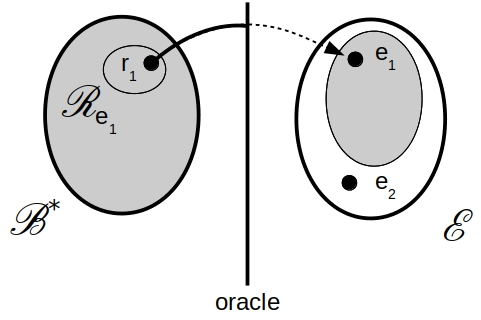
\includegraphics[scale=0.5]{entities_topics_1}
\caption{\label{fig:entities_topics_1}Encodings and Entities.}
\end{figure}

A consequence of working with finite strings as representations is that it might happen that there exist entities that are not encoded by any representation (see the gray areas in Figure \ref{fig:entities_topics_1}, in particular, the entity $e_2$ is not encoded by any representation). Intuitively, we could say that for some domains of knowledge the number of problems is much higher than the number of solutions.

\begin{example}
If the collection of entities under study are real numbers, it turns out that there exist numbers that can not be encoded using finite binary strings, since the set $\mathbb{R}$ has the cardinality of the continuum, and the set $\mathcal{B}^\ast$ is numerable.
\end{example}

Since our knowledge about the entities and the inner workings of the oracle are incomplete, in practice we will working with another set $\hat{\mathcal{R}}_e \subseteq \mathcal{B}^\ast$ of strings that we believe are close to the representations $\mathcal{R}_e$ that encode the entity $e$. The elements that belong to $\hat{\mathcal{R}}_e$ usually change over time, as we better understand the entities of $\mathcal{E}$, and how the oracle encode these entities as strings. The more abstract is our set of entities $\mathcal{E}$, the more difficult will be to approximate them as strings in $\hat{\mathcal{R}}_e$.

\begin{example}
\label{ex:luminiferous_ether}
The entity "luminiferous ether" was a theoretical postulate about a hypothetical medium in which the light would propagate. The ether was used as an explanation of how a wave-based light could propagate through the empty space. In 1887, the results of the Michelson-Morley experiment suggested that the ether did not exist, and after Einstein formulated his special theory of relativity, that successfully explained how light propagates through empty space, the idea of ether was completely dropped.
\end{example}

A consequence of working with approximations (the set $\hat{\mathcal{R}}_e$) instead of valid representations (the set $\mathcal{R}_e$) is that some of the candidate strings currently in use might encode a different entity from what we were expecting.

\begin{example}
\label{ex:polywater}
In 1961, the Soviet physicist Nikolai Fedyakin, performed a series of experiments resulting in what was seemingly a new form of water. The new water, called polywater, showed a higher boiling point, a lower freezing point, and much higher viscosity than ordinary water. Later experiment showed that polywater was nothing more than contaminated water with small amounts of impurities.
\end{example}

\begin{remark}
One of the problems of science, and in general of any human intellectual activity, is that people tend to confuse symbols with what they represent. The theory of nescience has been carefully designed to avoid this problem, by means of clearly stating the difference between research entities and the representation of entities. However, keeping this distinction always explicit in the explanations would make the book very difficult to read. We have tried to find a compromise between clarity in the exposition and rigor in the definitions. Sometimes, during the introduction of new ideas we talk in general about a \emph{topics}, meaning an entity, a representation, or both, an entity and its representation. But, in the mathematical definitions and propositions we always make this difference unequivocal. In case of doubt about what we mean, please take the mathematical definitions as the authoritative reference. 
\end{remark}

%
% Section: Joint Representations
%

\section{Joint Representations}
\label{sec:descriptions_joint_topic}

We have seen in the previous section that there exists more than one possible representation of an entity $e \in \mathcal{E}$, what we have called the set $\mathcal{R}_e$ of representations of the entity $e$. Some of these representations have a high quality, in the sense that they contain all the information required by the oracle to reconstruct (in whatever way the oracle manages to do that) the original entity. But also, in the set $\mathcal{R}_e$ there exists low quality representations, that is, representations that lack many of the details needed to fully reconstruct the entity. Furthermore, the set $\mathcal{R}_e$ can contain representations that include information that is sinply wrong, symbols that the oracle will ignore when reconstructing the original entity, but that will mislead us when understanding this entity. In Chapter \ref{chap:Miscoding} we will study in detail the errors due to incomplete and wrong representations.

If we want to increase our knowledge about an entity, we have to find the best possible representation for that entity, that is, a representation that is complete and correct. One way to do that is to simply try different strings until we come up with a high quality representation. However, that method could require a lot of time. A more efficient approach would be to complement our current bad representation with more (potentially missing) symbols, or by combining those known representations that contain partial information. These two methods require the introduction of the concept of joint representation.

\begin{definition}
Let $s, t \in \mathcal{B}^\ast$ be two different representations. We call the \emph{joint representation} of $s$ and $t$ to the concatenation string $st$.
\end{definition}

\begin{example}
\label{ex:lung_cancer}
Suppose that the research entity $e$ in which we are interested is the causes of lung cancer. In order to understand this entity, we have measured a collection of risk factors in a random sample of the population (smooking, exercise, diet, age, etc.). However, due to a problem with the sampling procedure, all the samples correspond to a subset of the population, for example, males. This dataset would be a representation $s$ for our entity $e$, but a very bad one, since it is biased. If we have a second representation, corresponding the sample data of females $t$, the joint representation $st$ will be a better one that any of them, $s$ or $t$, isolated.
\end{example}

The concatenation of any two arbitrary representations is also a representation.

\begin{proposition}
Let $s, t \in \mathcal{B}^\ast$ be two different representations and $st$ its joint representation, then $st$ is also a representation.
\end{proposition}
\begin{proof}
As we have seen in Section \ref{sec:strings} the set $\mathcal{B}^\ast$ is closed under the operation of concatenation of strings, and the representation function $\mathcal{O}_\mathcal{E}$ is total.
\end{proof}

We do not require the set of representations $\mathcal{R}_e$ for a given entity $e \in \mathcal{E}$ to be closed under the operation of concatenation. It might happen that $st \notin \mathcal{R}_e$, even if it is the case that $s \in \mathcal{R}_e$ and $t \in \mathcal{R}_e$.

The concept of joint representation is defined for every pair of strings $s, t \in \mathcal{B}^\ast$, even if they do not belong to the same set of representations $\mathcal{R}_e$, in other words, when $\mathcal{O}_\mathcal{E} \left( s \right) \neq \mathcal{O}_\mathcal{E} \left( t \right)$. This process of joining representations from different entities will be very usefull in the discovery of new research entities hitherto unknown (see Section \ref{sec:New_Research_Topics}), recall that all possible strings must represent an entity.

The operation of string concatenation is associative, that is, $(rs)t = r(st)$, for all $r, s, t \in \mathcal{B}^\ast$. This property defines the algebraic structure of the set of representations.

\begin{proposition}
The set $\mathcal{B}^\ast$ of representations together with the operation of concatenation has the structure of free monoid.
\end{proposition}
\begin{proof}
As we have seen in Section \ref{sec:strings} the operation of string concatenation in $\mathcal{B}^\ast$ is associative, and the empty string $\lambda$ plays the role of neutral element.
\end{proof}

We do no require the operation of joining representations to be conmutative with respect to the oracle function. Given the representations $s, t \in \mathcal{B}^\ast$ it might happen that the concatenation strings $st$ and $ts$ represent different entities, that is, $\mathcal{O}_\mathcal{E} \left( st \right) \neq \mathcal{O}_\mathcal{E} \left( ts \right)$.

The concept of joint representation can be extended to any arbitrary, but finite, collection of representations. In this way, we could add multiple partial representations to our research, or use them in the process of discovering new entities.

\begin{definition}
Let $r_1, r_2, \ldots, r_n \in \mathcal{B}^\ast$ be a finite collection of representations. We call the \emph{joint representation} of $r_1, r_2, \ldots, r_n$ to the string $r_1 r_2 \ldots r_n$.
\end{definition}

It is easy to show that $r_1 r_2 \ldots r_n \in \mathcal{B}^\ast$ for all $r_1, r_2, \ldots, r_n \in \mathcal{B}^\ast$, that is, $\mathcal{B}^\ast$ is closed under the operation of concatenation of multiple, finite, representations.

%
% Section: Descriptions
%

\section{Descriptions}
\label{sec:descriptions_models}

So far, our aim with the strings of $\mathcal{B}^\ast$ has been to provide an enconding, or representation, as complete and detailed as possible of the entities of $\mathcal{E}$, no matter its length. However, as we have said in the preface of this book, human understanding requires the derivation of concise models for those entities, since human reasoning cannot be based on long representations.

\begin{example}
In Example \ref{ex:lung_cancer} we have shown that a good representation for the entity "lung cancer" could be a sample dataset in which we measure different risk factors. If someone decides to quit smooking is not because they know and understand this large sample dataset, but because they know and understand the much simpler derived model "smooking increases the risk of lung cancer".
\end{example}

A description or model\footnote{In the theory of nescience use the words "description" and "model" interchangeably.} is a finite binary string mapped to a representation of an entity (recall Figure \ref{fig:entities_topics_models} from Chapter \ref{chap:Introduction}). Descriptions do not model entities (target systems) directly, they do so through string based representations.

In the theory of nescience we require that descriptions must be computable, so we can fully and effectively reconstruct the original representations given their descriptions. The requirement of computability allows us to clearly state the limits of the concept of "description". For example, the problem of self-referential descriptions, like the Berry paradox\index{Berry paradox}, can be addressed in the scope of the limits of computation.

\begin{definition} [Model]
\label{def:descriptions_model}
Let $d \in \mathcal{B}^\ast$ be a binary string in the form $d = \langle TM,a \rangle$, where $TM$ is the encoding of a prefix free Turing machine and $a$ is the input string to that machine. If $TM(a)$ is defined, we say that $d$ is a \emph{description}\index{Description}. 
\end{definition}

The output of the description $TM(a)$ is a string, that is, the representation of an entity. Intuitively, a description is composed by two parts, a Turing machine that compresses all the regularities found in this representation, and a string containing what is left, that is, the non-compressible part. From an otological point of view, descriptions are just string based representations that satisfy some additional requirements, like being computable. In this sense, descriptions are also representations themselves, i.e., the set of descriptions is a subset of the set of representations.

\begin{definition}
\label{def:descriptions_model}
We define the \emph{set of descriptions}\index{Set of descriptions}, denoted by $\mathcal{D}$, as:
\[
\mathcal{D} = \{ d \in \mathcal{B}^\ast : d = \langle TM,a \rangle \wedge TM(a) \downarrow \}.
\]
Let $r \in \mathcal{B}^\ast$ be a representation. We define the set of \emph{descriptions for $r$}, denoted by $\mathcal{D}_r$, as:
\[
\mathcal{D}_r = \{ d \in \mathcal{D} : TM(a) = r \}.
\]
Finally, given an entity $e \in \mathcal{E}$, we define the set of \emph{descriptions for $e$}, denoted by $\mathcal{D}_e$, as:
\[
\mathcal{D}_e = \{ d \in \mathcal{D} : \exists r \in \mathcal{R}_e,\, TM(a) = r \}.
\]
\end{definition}

Given that descriptions are representations themselves, there exists descriptions that describe descriptions. From a practical point of view it is not a good idea to use descriptions as the representation of entities, since what we are looking for in a good representation is that they contain as much inforformation as possible about the original entities, not an encoding as concise as possible. Working with descriptions in the role of representations would make the job of scientific discovery very difficult.

\begin{notation}
In case of dealing with multiple represenations and descriptions, and in order to avoid ambiguity, we will denote by $d_r$ the description $d$ for the representation $r$.
\end{notation}

Since each description describes one, and only one, representation, we can define a function that maps descriptions into representations. Given that descriptions are Turing machines, it is natural to use as description function a universal Turing machine. Consequently, not only the individual descriptions of representations are computable, but also the function that maps descriptions into representations is computable.

\begin{definition}
We call \emph{description function}\index{Description function}, denoted by $\delta$, to any universal Turing machine $\delta : \mathcal{D} \rightarrow \mathcal{B}^\ast$ that maps descriptions to their corresponding representations.
\end{definition}

If $d$ is a description of the representation $r$, then we have that $\delta \left( d \right) = \delta \left( \langle TM, a \rangle \right) = TM(a) = r$.

Inspired by the Occam's razor principle\index{Occam's razor principle}\footnote{The Occam's razor principle refers to the number of assumptions of an explanation, not to the length of the explanation itself.}, if two explanations are indifferent, we should prefer the shortest one. Therefore, the limit of what can be known (understand) about a representation, that is, its perfect model, is given by the shortest description that allows us to reconstruct this representation. Of course, what we know about the original entity is conditional to the quality of the representation.

\begin{definition}
\label{def:descriptions_perfect_model}
Given the set of descriptions $\mathcal{D}_r$ of a representaton $r \in \mathcal{B}^\ast$, let $d_r^{\star} \in \mathcal{D}_r$ be the shortest possible description of $r$ using the standard shortlex ordering. We call $d_r^{\star}$ the \emph{perfect description}\index{Perfect description} of the representation $r$.
\end{definition}

Unfortunately, the perfect description of a representation is in general not known and, as Proposition \ref{prop:nescience-kolmogorov} shows, there exist no algorithm to compute it. In practice what we have to do is to use an approximation to estimate how far our current best description is from the perfect one, that is, how much we do not know about a particular representation for an entity (see Chapter \ref{chap:Redundancy}).

\begin{proposition}
\label{prop:nescience-kolmogorov}
Given a representation $r \in \mathcal{B}^\ast$, we have that $l \left( d_r^{\star} \right) = K\left( r \right)$.
\end{proposition}
\begin{proof}
Apply Definition \ref{def:Kolmogorov-Complexity} and the fact that we require that the Turing machines $TM$ used in definitions $\langle TM,a\rangle$ must be prefix-free.
\end{proof}

The actual length of a description $l \left( d \right)$ for a representation $r$ is something that depends on the particular enconding of Turing machines used. The encoding method is given by the description function $\delta$ used. Fortunately, if we replace our description function by a different one, the length of perfect models do not change (up to an additive constant that does not depend on the representations themselves).

\begin{corollary}
Let $r \in \mathcal{B}^\ast$ be a representation, $\delta$ and $\dot{\delta}$ two different description functions, and $d_r^{\star}$ the perfect description of the representation $r$ using $\delta$ and $\dot{d}_r^{\star}$ the perfect description using $\dot{\delta}$, then we have that $l \left( d_r^{\star} \right) \leq l \left( \dot{d}_r^{\star} \right) + c$ where $c$ is a constant that does not depend on $r$.
\end{corollary}
\begin{proof}
Apply Theorem \ref{prop:nescience-kolmogorov} and Theorem \ref{def:Invariance-theorem}.
\end{proof}

In general, in the theory of nescience we are not interested in computing the actual value of the nescience about an entity given a description and a representation. Instead what we are interested is in the ordering of the different possible pairs of descriptions and representations given their nescience. In this sense, the details of the particular universal Turing machine used in practice are not relevant\footnote{Do not confuse the inner workings of the universal Turing machine that maps descriptions to representations, in which we are not interested, with the inner workings of the universal oracle Turing machine that maps representations to entities, in which we are interested, since this knowledge is critical to understand how things work.}. For the rest of this book we will assume that $\delta$ is fixed to a reference universal Turing machine. For example, in Section \ref{sub:ax_type_theory} we use as univeral Turing machine the lambda calculus. Alternatively, the reader could consider that all the theorems provided in this book that deal with the length of shortest models are valid up to an additive constant that does not depend on the topics themselves.

A remarkable consequence of Proposition \ref{prop:nescience-kolmogorov} is that perfect descriptions must be incompressible, that is, \emph{perfect knowledge implies randomness} (see Section \ref{sec:incompressibility_randomness}).

\begin{corollary}
Let $d_r^{\star}$ be the perfect description of a representation $r$, then we have that $K \left( d_r^{\star} \right) = l \left( d_r^{\star} \right)$.
\end{corollary}
\begin{proof}
Having $K \left( d_r^{\star} \right) < l \left( d_r^{\star} \right)$ would be a contradiction with the fact that $d_r^{\star}$ is the shortest possible description of $r$.
\end{proof}

The converse, in general, does not hold, since we could have a random description that it is not the shortest possible one, that is, a description $d$ for a reprsentation $r$ such that $l(d) = K(d)$ but $l(d_r^{\star}) < l(d)$.

\begin{example}
\label{ex:description_neural}
We could define a deep neural network\index{Neural network} with an input layer of one thousands nodes, ten hidden layers of fifty thousands nodes each, and an output layer of one thousand nodes, and then train the network to output a fixed string of one thousand 1's for any given input string. The Kolmogorov complexity of this neural network is much higher that the complexity of a string of one thousand 1's.
\end{example}

There is little value on a descriptions that is longer than the representation it describes.

\begin{definition}
\label{def:trivial_model}
Let $r \in \mathcal{B}^\ast$ be a representation, and $d \in \mathcal{D}_r$ one of its descriptions. If $l(d) \geq l(r)$, we say that $d$ is a \emph{pleonastic description}\index{Pleonastic description} of the representation $r$.
\end{definition}

\begin{example}
\label{ex:topics_models_graph}
Consider the set of all possible finite graphs\index{Graph}. Since graphs are abstract mathematical objects, we need a way to represent them as strings, for example, by using a binary encoding of their adjacency matrices (see Section \ref{sec:Graphs} for an introduction to graphs). The description $d = \langle TM, r \rangle$, where $r$ is the representation of a graph and $TM$ is a Turing machine that just halts, will be part of $\mathcal{D}_r$ since $TM(r) = r$. We are concerned about the fact that this description may not be shortest possible description of $r$.
\end{example}

It might happen that there is no shortest possible description of a representation than the representation itself. This is the case when representations are random, or incompressible, strings. And, as we have seen in Section \ref{sec:incompressibility_randomness} the overhelming majority of strings are incompressible. It does not make any sense to do research about random representation, since it is not possible to find shorter models for that representation.

The concept of perfect description can be generalized from individual representations to entities. This generalization allow us to study the nature and properties of these entities.

\begin{definition}
\label{def:entities_perfect_model}
Given the set of descriptions $\mathcal{D}_e$ of an entity $e \in \mathcal{E}$, let $d_e^{\star} \in \mathcal{D}_e$ be the shortest possible description of $\mathcal{D}_e$ using the standard shortlex ordering. We call $d_e^{\star}$ the \emph{perfect model}\index{Perfect model} of entity $e$.
\end{definition}

For each possible representation $r$ of $e$ we can compute its perfect description $d_r^{\star}$. Then, the perfect description $d_e^{\star}$ for $e$ would be the shortest of this collection of perfect descriptions of the representations.

An interesting case is when all the descriptions that compose $\mathcal{D}_e$ are pleonastics, that is, there is no model that it is shorter than the representation for all the possible representations of the entity. That would the case if all the representations of the entity $e$ are random strings. In this particular case, scientific research would be doomed, since it is not possible to find a suitable model for $e$. The fact that we can understand and make predictions about $e$ will be limited by the length of the non-compressible representations of $e$.

{\color{red} Elaborate a little bit more over the concept of perfect description of an entity.}

%
% Section: Models for Joint Representations
%

\section{Descriptions for Joint Representations}
\label{sec:description_joint_represenation}

In Section \ref{sec:descriptions_joint_topic} we introduced the concept of joint representation $ts$ of two individual representations $t$ and $s$. In this section we are interested in to study how the length of the optimal description of a joint representation relates to the length of the optimal descriptions of the individual representations.

The length of the perfect description of a joint representation is greater or equal than the length of the perfect description of any of the individual representations. That is, the more information we include in a representation, the longer will take to describe it. 

\begin{proposition}
\label{prop:joint_length}
Given any two representations $t,s \in \mathcal{B}^\ast$, we have that $l \left( m_{ts}^{\star} \right) \geq l \left( m_{t}^{\star} \right)$ and $l \left( m_{ts}^{\star} \right) \geq l \left( m_{s}^{\star} \right)$, where $m_{t}^{\star}$, $m_{s}^{\star}$ and $m_{ts}^{\star}$ are the perfect descriptions of the representatons $t$, $s$ and the joint representation $ts$ respectively.
\end{proposition}
\begin{proof}
The statement $l \left( m_{ts}^{\star} \right) \geq l \left( m_{t}^{\star} \right)$ is equivalent to $K(t,s) \geq K(t)$. Then apply Proposition \ref{prop:excess_kolmogorov}.
\end{proof}

Intuitively, adding more information to a representation is a good thing if this information is relevant to describe the entity in which we are interested. But adding non-relevant information will make our model unnecessarily long.

If the selected two representations partially overlap, we could take advantage of this fact to come up with a shorter description. In the worst case, the perfect description of a joint represenation would be just the concatenation of the perfect descriptions of the involved representations.

\begin{proposition}
\label{prop:joint_sum}
Given any two topics $t,s \in \mathcal{T}$, we have that $l \left( m_{ts}^{\star} \right) \leq l \left( m_{t}^{\star} \right) + l \left( m_{s}^{\star} \right)$.
\end{proposition}
\begin{proof}
The statement $l \left( m_{ts}^{\star} \right) \leq l \left( m_{t}^{\star} \right) + l \left( m_{s}^{\star} \right)$ is equivalent to $K(t,s) \leq K(t) + K(s)$, then apply Proposition \ref{prop:additive_kolmogorov}.
\end{proof}

Another interpretation of the above proposition would be to consider a representation $r$ that is the concatenation of two, partially overlapping, representations $s$ and $t$, that is, $r = st$. In this sense, Proposition \ref{prop:joint_sum} says that including redundant information in a description is not a problem from the proint of view of finding the shortes possible description. Compare with Proposition \ref{prop:joint_length} that states that adding non-relevant information to a representation is a bad thing.

Finally, next proposition proves that the order of the representations in the perfect description of a joint representation does not change its length.

\begin{proposition}
\label{prop:joint_order}
Given any two representations $t, s \in \mathcal{B}^\ast$, we have that $l \left( m_{ts}^{\star} \right) = l \left( m_{st}^{\star} \right) + c$.
\end{proposition}
\begin{proof}
The statement $l \left( m_{ts}^{\star} \right) = l \left( m_{st}^{\star} \right) + c$ is equivalent to $K(ts) = K(st) + c$, then apply Proposition \ref{prop:kolmogorov_order}.
\end{proof}

Of course, given the concatenated $ts$ we cannot infer the original $t$ and $s$, since they are not self-delimited repsentations. But this fact is not relevant to the problem of finding the shortest possible description of the concatenated string.

Propositions \ref{prop:joint_length}, \ref{prop:joint_sum} and \ref{prop:joint_order} can be generalized to any arbitrary, but finite, collection of representations $t_1, t_2, \ldots, t_n$.

\begin{proposition}
\label{prop:joint_multiple_topics}
Let $t_1, t_2, \ldots, t_n \in \mathcal{T}$ be a finite collection of representations. Then, we have that:

\renewcommand{\theenumi}{\roman{enumi}}
\begin{enumerate}
\item $l(m_{t_1 t_2 \ldots t_n}^\star) \geq l(m_ {t_i}^\star) \; \forall \, 0 \leq i \leq n$,
\item $l(m_{t_1 t_2 \ldots t_n}^\star) \leq l(m_ {t_1}^\star) + l(m_ {t_2}^\star) + \ldots + l(m_ {t_n}^\star)$,
\item $l(m_{t_1 \ldots t_i \ldots t_j \ldots t_n}^\star) = l(m_{t_1 \ldots t_j \ldots t_i \ldots t_n}^\star) + c \; \forall \, 0 \leq i \leq j \leq n$,
\item $l(m_{t_1 \ldots t_{n-1}}^\star) \leq l(m_{t_1 \ldots t_{n-1} t_n}^\star)$.
\end{enumerate}
\end{proposition}
\begin{proof}
Apply Propositions \ref{prop:joint_length}, \ref{prop:joint_sum} and \ref{prop:joint_order} to individual pairs of topics $i$ and $j$.
\end{proof}

%
% Section: Conditional Descriptions
%

\section{Conditional Descriptions}

Sometimes it is cumbersome to include all the information needed to reconstruct an entity in its description, since that would require very large strings. In those cases, it is usually more convenient to assume some already existing background knowledge, and compute how much we do not know about an entity given that background, what we call \emph{conditional descriptions}. Conditional descriptions also play a very important role in the discovery of new knowledge: if by conditioning a description on some prior knowledge we manage to significantly reduce the inaccuracy, that would mean this prior knowledge is important for understanding the entity.

\begin{definition}
Let $r, d, s \in \mathcal{B}^\ast$ be strings. We say that the string $\langle d, s \rangle$ is a \emph{valid conditional description}\index{Conditional model} of the representation $r$ given the string $s$, denoted by $d \mid s$, if $d$ is a description $\langle TM, a \rangle$, and $TM \left(\langle a, s \rangle \right) = r$.
\end{definition}

The conditional description $\langle d, s \rangle$ is based on two strings $a$ and $s$, that play very different roles. The string $a$ is the input to the Turing machine $TM$,  and it should contain the non-compresible part of the representation $r$. The string $s$ should be the description, or representation, of another entity whose knowledge can helps to understand the entity in which we are interested. For example, as we will see in Chapter \ref{chap:Redundancy}, the string $s$ is not taken into account when computing the surfeit of a conditional description.

Note that the conditional description $d \mid s$ does not belong to the set of valid description $\mathcal{D}^\star_r$ for the representation $r$, since $s$ is required to compute the representation $r$, but it is not part of the description itself. A new definition is required to capture this concept.

\begin{definition}
Let $r \in \mathcal{B}^\ast$ be a representation and $s \in \mathcal{B}^\ast$ an arbitrary string, we define the \emph{set of conditional descriptions}\index{Set of conditional descriptions} of $r$ given $s$, denoted by $\mathcal{D}_{r \mid s}^\star$, as:
\[
\mathcal{D}_{r \mid s}^\star = \{ d \in \mathcal{D}, d = \langle TM, a \rangle : TM \left(\langle a, s \rangle \right) = r \}.
\]
\end{definition}

For each representation $r \in \mathcal{B}^\ast$ there always exists a conditional description $d \mid s$ that describes $r$, as next proposition shows.

\begin{proposition}
Let $r \in \mathcal{B}^\ast$ be a representation and $s \in \mathcal{B}^\ast$ an arbitrary string. If $d \in \mathcal{D}_{r}^\star$ then $d \in \mathcal{D}_{r \mid s}^\star$.
\end{proposition}
\begin{proof}
We can use a conditional description $\langle \langle TM, a \rangle, s \rangle$ based on a Turing $TM$ machine that given the input $\langle a, s \rangle$ safely ignores the $s$ string.
\end{proof}

We are interested in the concept of perfect conditional description. The perfect conditional description of a representation given a prior knowledge is the shortest possible string that allow us to fully reconstruct the representation assuming this prior knowledge.

\begin{definition}
Let $r \in \mathcal{B}^\ast$ be a representation, and let $d^\star \mid s$ be the shortest possible description of $r$ given the string $s$. We call $d^\star \mid s$ the \emph{perfect conditional description} of the representation $r$ given the string $s$, or perfect conditional description of $r$ given $s$ for short.
\end{definition}

The length of perfect conditional description is equal or shorter that their unconditional counterparts. That is, assuming some already existing background knowledge could reduce the effort required to describe a representation.

\begin{proposition}
\label{prop:description_conditional_inequality}
For any representation $r \in \mathcal{B}^\ast$ we have that $l \left( d^\star \mid s \right) \leq l \left( d^\star \right)$ for all $s \in \mathcal{B}^\ast$.
\end{proposition}
\begin{proof}
The statement $l \left( d^\star \mid s \right) \leq l \left( d^\star \right)$ is equivalent to $K(r \mid s) \leq K(r)$, then apply Proposition \ref{prop:kolmogorov_conditional}.
\end{proof}

Next proposition shows the relation between the lengths of descriptions, join descriptions and conditional descriptions.

\begin{proposition}
\label{prop:description_conditional_joint}
Let $r, s \in \mathcal{B}^\ast$ two different representations. We have that:
\[
l \left( d^\star_{r \mid s} \right) \leq l \left( d^\star_r \right) \leq l \left( d^\star_{rs} \right)
\]
\end{proposition}
\begin{proof}
The statement $l \left( d^\star_{r \mid s} \right) \leq l \left( d^\star_r \right) \leq l \left( d^\star_{rs} \right)$ is equivalent to $K(r | s ) \leq K(r)$ and $K(r) \leq K(r, s)$, then apply Proposition \ref{prop:kolmogorov_relations}.
\end{proof}

As it was the case of joint descriptions, the concept of conditional description can be extended to finite collections of topics.

\begin{definition}
Let $r, d, s_1, s_2, \ldots, s_n \in \mathcal{B}^\ast$ be strings. We say that the string $\langle d, s_1, s_2, \ldots, s_n \rangle$ is a \emph{valid conditional description}\index{Conditional model} of the representation $r$ given the strings $s_1, s_2, \ldots, s_n$, denoted by $d \mid s_1, s_2, \ldots, s_n$, if $d$ is a description $\langle TM, a \rangle$, and $TM \left(\langle a, s_1, s_2, \ldots, s_n \rangle \right) = r$.
\end{definition}

In the next definition we provide the generalization of the concept of perfect conditional descriptions.

\begin{definition}
Let $r \in \mathcal{B}^\ast$ be a representation, and let $d^\star \mid s_1, s_2, \ldots, s_n$ be the shortest possible description of $r$ given the strings $s_1, s_2, \ldots, s_n$. We call $d^\star \mid s_1, s_2, \ldots, s_n$ the \emph{perfect conditional description} of the representation $r$ given the string $s_1, s_2, \ldots, s_n$, or perfect conditional description of $r$ given $s_1, s_2, \ldots, s_n$ for short.
\end{definition}

Next proposition generalizes Propositions \ref{prop:description_conditional_inequality} and \ref{prop:description_conditional_joint} to any arbitrary, but finite, collection of strings $s_1, s_2, \ldots, s_n$. Moreover, the proposition shows that the more background knowledge we assume for a representation, the shorter is the perfect description for that representation.

\begin{proposition}
Let $r, s_1, s_2, \ldots, s_n \in \mathcal{B}^\ast$ be a finite collection of strings. Then, we have that:
\[
l \left( d^\star_{r \mid s_1, s_2, \ldots, s_n} \right) \leq l \left( d^\star_r \right) \leq l \left( d^\star_{r,s_1, s_2, \ldots, s_n} \right)
\]
\end{proposition}
\begin{proof}
{\color{red} TODO Review} Apply Propositions \ref{prop:description_conditional_inequality} and \ref{prop:description_conditional_joint} to individual pairs of representations $i$ and $j$.
\end{proof}

{\color{red} TODO: Introduce the following proposition.}

\begin{proposition}
Let $r, s_1, s_2, \ldots, s_n, s_{n+1} \in \mathcal{B}^\ast$ be a finite collection of strings. Then, we have that:
\[
l \left( d^\star_{r \mid s_1, s_2, \ldots, s_n, s_{n+1}} \right) \leq l \left( d^\star_{r \mid s_1, s_2, \ldots, s_n} \right)
\]
\end{proposition}
\begin{proof}
{\color{red} TODO Review} Apply Propositions \ref{prop:description_conditional_inequality} and \ref{prop:description_conditional_joint} to individual pairs of representations $i$ and $j$.
\end{proof}

%
% Section: Areas
%

\section{Research Areas}
\label{sec:areas}

Entities can be grouped into research areas. The concept of area is useful as long as all the entities included in the area are related to a common knolewdge subdomain. The particular details of the grouping criteria depend on the practical applications in which the theory of nescience is being used.

\begin{definition}
Given a set of entities $\mathcal{E}$, we define a \emph{research area}\index{Research area} $\mathcal{A}$ as a subset of entities $\mathcal{A} \subset \mathcal{E}$.
\end{definition}

If we want to know how much we do not know about a research area, first we have to provide a representation for that area. In general areas are infinite, but the number of known representations is finite, and so, we can only describe the areas with respect to our current knowledge.

\begin{definition}
Let $A \subset \mathcal{E}$ be an area. We define the \emph{known subset of the area}\index{Known subset of an area} $\mathcal{A}$, denoted by $\hat{\mathcal{A}}$, as the set composed by those entities $e_1, e_2, \ldots, e_n \in A$ for which at least one non-trivial model is known.
\end{definition}

We have to distinguish between the knowable subset of $\mathcal{A}$, composed by those entities for which there exists a representation, and the know subset of $\mathcal{A}$, composed by those entities for which we know a non-trivial model, that is, those entities for which somebody has already done some research about them. Of course, the set of known entities is a subset of the set of knowable entities.

As our understanding of a research area changes, the number of entities included in its known subset changes as well. The properties of areas studied in this book will be always relative to our current knowledge.

\begin{definition}
Let $\mathcal{A} \subset \mathcal{E}$ be an area with known subset $\hat{\mathcal{A}} = \{ e_1, e_2, \ldots, e_n \}$, and let  $R = \{ r_1, r_2, \ldots, r_n \}$ a set of representations, such that $r_i \in \mathcal{R}_{e_i}$. We call $R_{\hat{\mathcal{A}}}$ a \emph{representation of the area $\mathcal{A}$} given the known subset $\hat{\mathcal{A}}$, abbreviated as \emph{representation of $A$}.
\end{definition}

In the same way, we can introduce the concept of description of an area.

\begin{definition}
Let $R_{\hat{\mathcal{A}}} = \{ r_1, r_2, \ldots, r_n \}$ be the representation of an area $\mathcal{A}$. We call a \emph{description of the area $\mathcal{A}$} given the known subset $\hat{\mathcal{A}}$, abbreviated as \emph{description of $\mathcal{A}$}, and denoted by $d_{\hat{\mathcal{A}}}$, to any string in the form $\langle TM, a\rangle$ such that $TM(a) = \langle r_1, r_2, \ldots, r_n\rangle$.
\end{definition}

We can also define the set of descriptions of an area.

\begin{definition}
Let $R_{\hat{\mathcal{A}}} = \{ r_1, r_2, \ldots, r_n \}$ be the representation of an area $\mathcal{A}$. We define the set of \emph{descriptions for $R_{\hat{\mathcal{A}}}$}, denoted by $\mathcal{D}_{R_{\hat{\mathcal{A}}}}$, as:
\[
\mathcal{D}_{R_{\hat{\mathcal{A}}}} = \{ d \in \mathcal{D} : TM(a) = \langle r_1, r_2, \ldots, r_n\rangle \}.
\]
\end{definition}

Finally, we are interested in the perfect model for a research area, that is, the shortest possible string that fully describes its known subset. According to Definition \ref{def:trivial_model}, if we are aware of the existence of a entity $e \in A$, that entity should be part of $\hat{A}$, even in the case we have not started yet to do research about that particular topic.

\begin{definition}
Let $A \subset \mathcal{E}$ be an area with known subset $\hat{A}$, and let $d_{\hat{A}}^{\star} \in \mathcal{M}_{\hat{A}}$ be the shortest possible description of $A$. We call  $d_{\hat{A}}^{\star}$ the \emph{perfect description of the area $A$} given the known subset $\hat{A}$\index{Perfect description of an area}, abbreviated as \emph{perfect description of $A$}.
\end{definition}

Next proposition shows the relation between the description of an area, and the descriptions of the entities that compose the known subset of that area. In general, the models for an area are different from the collection of models of the individual topics.

\begin{proposition}
Let $A \subset \mathcal{E}$ be an area with known subset $\hat{A} = \{e_1, e_2, \ldots, e_n\}$, then we have that $l \left( d_{\hat{A}}^{\star} \right) \leq l(d_ {e_1}^\star) + l(d_ {e_2}^\star) + \ldots + l(d_ {e_n}^\star)$.
\end{proposition}
\begin{proof}
Apply Proposition \ref{prop:joint_multiple_topics}-ii. 
\end{proof}

Also, as it was proved in Proposition \ref{prop:joint_multiple_topics}, the order in which the representations are listed in the description of an area is not relevant when dealing with the perfect model for that area.

Areas can overlap, that is, given two areas $A$ and $B$ it might happen that $A \cap B \neq \varnothing$. Moreover, areas can be subsets of other areas, creating an hierarchy of areas. We are interested in the length of perfect models of areas in relation to the length of perfect models of other areas.

\begin{proposition}
Let $A, B \subset \mathcal{E}$ be two areas such that $A \subset B$, and let $\hat{A}$ and $\hat{B}$ be their know subsets respectively, then we have that $l \left( d_{\hat{A}}^{\star} \right) \leq l \left( d_{\hat{B}}^{\star} \right)$.
\end{proposition}
\begin{proof}
{\color{red} TODO}
\end{proof}

Next proposition \label{prop:areas_union} shows how the length of the shortest possible description of areas relate to the union and intersection of such areas.

\begin{proposition}
\label{prop:areas_union}
Let $A, B \subset \mathcal{E}$ be two areas with know subsets $\hat{A}$ and $\hat{B}$ respectively, then we have that $l \left( d_{\hat{A} \cup \hat{B}}^{\star} \right) = l \left( d_{\hat{A}}^{\star} \right) + l \left( d_{\hat{B}}^{\star} \right) - l \left( d_{\hat{A} \cap \hat{B}}^{\star} \right)$.
\end{proposition}
\begin{proof}
{\color{red} TODO}
\end{proof}

A consequence of Proposition \label{prop:areas_union} is that $l \left( d_{\hat{A} \cup \hat{B}}^{\star} \right) \leq l \left( d_{\hat{A}}^{\star} \right) + l \left( d_{\hat{B}}^{\star} \right)$, that is, when we combines two different research areas, how much we do not know about these areas decreases.

In the same way we introduced a chain rule for entropy in Proposition \ref{prop:chain_rule_entropy}, we can provide a chain rule for the shortest length for a description of a research area.

\begin{proposition}
Let $A, B \subset \mathcal{E}$ be two areas with know subsets $\hat{A}$ and $\hat{B}$, then we have that $l \left( d_{\hat{A} \cup \hat{B}}^{\star} \right) = l \left( d_{\hat{A}}^{\star} \right) + l \left( d_{\hat{B} \backslash \hat{A}}^{\star} \right)$.
\end{proposition}
\begin{proof}
{\color{red} TODO}
\end{proof}

%
% Section: References
%

\section{References}

{\color{red} TODO: Review this section.}

For more information about Russell's paradox, Cantor theorem and universal sets refer, for example, to \cite{jech2013set}. The idea of using a function to assigns to each symbol and well-formed formula of some formal language a unique natural number (Gödel number) was introduced by Kurt Gödel for the proof of his incompleteness theorems \cite{godel1931formal}. A detailed description of the Berry paradox from the point of view of computability can be found at \cite{chaitin1995berry}. For a detailed account of the implications of Kolmogorov complexity being true up to a constant, please refer to \cite{li2013introduction}. That oracle machines are not mechanical was stated by Turing when he introduced the concept of oracle machine in \cite{turing1939systems}.

\begin{itemize}
\item Intro to ontology: the things we can know about
\item Intro to epistemology: the problem of representation
\item What it is a representtaion: reference to oxford philosophy article
\item Reference to the concept of what it is research topic
\item The problem of representation in Kolmogorov complexity
\item Godel numbering
\item single, unique, physical world -> what it is thing called
\item Cantor theorem
\item Rusell paradox
\item Oracle Turing machine
\item ptolomeo and tycho
\end{itemize}

\emph{universal oracle machine}

Should be require the oracles to be minimal?